% \documentclass[12pt,handout,xcolor=pdftex,dvipsnames,table]{beamer} %For handouts.
\documentclass{beamer}
%\usepackage{pgfpages} %For handouts.
% This is the file main.tex
% \usepackage{handoutWithNotes}
\usepackage{subcaption} % subfigure
\usepackage{hyperref}
\usepackage{graphicx}
\usepackage[en-US]{datetime2} % fix warning of \author[*]{\today}
\usepackage{lmodern}% http://ctan.org/pkg/lm (For special Fonts)
\usepackage{ragged2e} % justify document
\usepackage{smartdiagram}
\usepackage{tikz}
\usetikzlibrary{shapes.geometric, arrows}
\tikzstyle{startstop} = [rectangle, rounded corners, minimum width=3cm, minimum height=1cm,text centered, draw=black, fill=red!30]
\tikzstyle{io} = [trapezium, trapezium left angle=70, trapezium right angle=110, minimum width=3cm, minimum height=1cm, text centered, draw=black, fill=blue!30]
\tikzstyle{process} = [rectangle, minimum width=3cm, minimum height=1cm, text centered, draw=black, fill=orange!30]
\tikzstyle{decision} = [diamond, minimum width=3cm, minimum height=1cm, text centered, draw=black, fill=green!30]
\tikzstyle{arrow} = [thick,->,>=stealth]
% \usepackage{subfig}

\mode<presentation>
\setbeamertemplate{blocks}[rounded][shadow=true]
\usetheme{Dresden} % so so
\setbeamertemplate{page number in head/foot}[totalframenumber]
\setbeamertemplate{navigation symbols}{} %take out the navigation symbols
\setbeamertemplate{caption}[numbered] %enumerate the caption and tables
\usefonttheme[stillsansseriflarge]{structureitalicserif}
  
%\mode<handout>{\setbeamercolor{background canvas}{bg=black!5}} %For handouts.
% \pgfpagesuselayout{4 on 1 with notes}[a4paper,border shrink=5mm]
  
%\makeatletter %reset the numbering on the subfigures (1)
%\@addtoreset{subfigure}{figure} %reset the numbering on the subfigures (2)
%\makeatother %reset the numbering on the subfigures (3)

%For Large figures
%\includegraphics[width=\linewidth,height=\textheight,keepaspectratio]{SMS}

\title{Kubernetes Vagrant CI / CD} % (optional, only for long titles)
\subtitle{
	\href{https://github.com/thanos1983/kubernetesVagrant}
    		{GitHub Project Repo: kubernetesVagrant}
}
\author[Athanasios Garyfalos]{Sample of Work of fully automate build, deploy, validate containers locally. Deploy on a k8s cluster and validations.} % (optional, for multiple authors)
% {A.~Garyfalos \and A.~Garyfalos2 \and A.~Garyfalos3}
\institute[garyfalos@cpan.org] % (optional)
{
	\\
	\medskip
	{
	% \emph{A.atga12@student.bth.se}
	% \emph{Another Author email}
	% \emph{Another Author}
	}
}
% \vspace*{-11.5em}
% \date{Date: \today}
% \subject{Sample of Work Demonstration Django Rest Framework}

\begin{document}
	\begin{frame}[noframenumbering]
  \begin{center}
    % Upper part of the page
    \includegraphics[width=.8\textwidth]{png/kubernetesLogo}\\ % [0.3cm]
  \end{center}
  \titlepage
\end{frame}

	% \include{./copyRightDisclaimer/copyRightDisclaimer}
	% \section*{Contents}
\begin{frame}[allowframebreaks]{Outline}
  \setbeamercovered{dynamic} % Makes the text appear before it presents nice!!!
  \tableofcontents[pausesections, sections={1-4}]
    \framebreak
  \tableofcontents[pausesections, sections={4-8}]
\end{frame}

	% \section{Introduction} \label{sec:k8sFuntamentals}
\subsection{Container Runtime Interface(s)}
\subsubsection{Docker}
\subsubsection{Podman}
\subsubsection{CRI-O}

\begin{frame}{High level description}
\setbeamercovered{dynamic}%Makes the text appear before it presents nice!!!!
	\begin{columns}[T] % contents are top vertically aligned
		\begin{column}{5cm} % each column can also be its own environment
			\begin{itemize}
				\item<+-| alert@+> VM Vs Container.
				\item<+-| alert@+> What is a Pod (pea pod)?
				\item<+-| alert@+> Container Runtime Interface(s) (CRI).
					\begin{itemize}
						\item<+-| alert@+> Docker
						\item<+-| alert@+> Podman
						\item<+-| alert@+> CRI-O
					\end{itemize}
				\item<+-| alert@+> Docker Vs Podman.
				\item<+-| alert@+> What is actually k8s?
			\end{itemize}
		\end{column}
		\begin{column}{5cm} % alternative top-align that's better for graphics
		\begin{figure}
			\only<1>{%
				\centering Virtual Machine Vs Container
				\includegraphics[width=\columnwidth, height=0.5\textheight]{./png/container}
			}%
			\only<2>{%
				\centering Container inside Pod
				\includegraphics[width=\columnwidth, height=0.5\textheight]{./png/pod}
			}%
			\only<3>{%
				\centering Container Runtime Interface
				\includegraphics[width=\columnwidth, height=0.5\textheight]{./png/cri}
			}%
			\only<4>{%
				\centering Most known (insecure) socket
				\includegraphics[width=\columnwidth, height=0.5\textheight]{./png/docker}
			}%
			\only<5>{%
				\centering Most unknown (secure) socket
				\includegraphics[width=\columnwidth, height=0.5\textheight]{./png/buildah-podman}
			}%
			\only<6>{%
				\centering Lightest fastest socket
				\includegraphics[width=\columnwidth, height=0.5\textheight]{./png/crio}
			}%
			\only<7>{%
				\centering Read about it
				\includegraphics[width=\columnwidth, height=0.5\textheight]{./png/dockervspodman}
			}%
			\only<8>{%
				\centering Is a puzzle of elements
				\includegraphics[width=\columnwidth, height=0.5\textheight]{./png/k8sPuzzle.jpg}
			}%
			\caption{k8s Overview} \label{fig:largeFigure}
		\end{figure}
		\end{column}
	\end{columns}
\end{frame}

	% \section{CI / CD} \label{sec:k8sVagrant}
\subsection{Project smooth CI / CD}

\begin{frame}{Problems / Desires / Solutions on CI / CD}
	\setbeamercovered{dynamic} %Makes the text appear before it presents nice!!!!
	\vspace{-0.4cm}
	\begin{columns}[T] % contents are top vertically aligned
		\begin{column}{5cm} % each column can also be its own environment
			\begin{block}{Assessment Requirements}
				\begin{itemize}
					\item<1-| alert@+> CI / CD (Locally / Remotely).
					\item<2-| alert@+> Everything As a Code
					\item<3-| alert@+> Validation Locally!!!
					\item<4-| alert@+> OS / Inf. dependencies.
				\end{itemize}
			\end{block}
		\end{column}
		\begin{column}{5cm} % alternative top-align that's better for graphics
			\begin{block}{Justification of Requirements}
				\begin{itemize}
					\item<1-| alert@+> Works on my PC, why not on Cloud?
					\item<2-| alert@+> Human error (manual).
					\item<3-| alert@+> Test (automatically).
					\item<4-| alert@+> GitHub Actions, Jenkins
				\end{itemize}
			\end{block}
		\end{column}
	\end{columns}
	\only<5-8>{%
	\begin{block}{Solutions to Requirements}
		\begin{itemize}
			\item<5-| alert@5> Solution has to be reproducible locally. \alert{Exactly as cloud}.
			\item<6-| alert@6> Minimal human interaction. Auto \alert{error handling} (Rollback)!
			\item<7-| alert@7> \alert{Powerful PCs!} (8 CPUs / 35 GB RAM). Browsing (tabs)?
			\item<8-| alert@8> \alert{No Vendor binding} (Azzure DevOps, Jenkins, Bamboo etc).
		\end{itemize}	
	\end{block}
	}%
\end{frame}

\subsection{How to accomplish requirements}

\begin{frame}{Solution to problem}
	\setbeamercovered{dynamic} %Makes the text appear before it presents nice!!!!
	\begin{alertblock}{Problems}
		\begin{itemize}
			\item<1-| alert@1> Solution has to be reproducible locally. \alert{Exactly as cloud}.
			\item<2-| alert@2> Minimal human interaction. Auto \alert{error handling} (Rollback)!
			\item<3-| alert@3> \alert{Powerful PCs!} (8 CPUs / 35 GB RAM). Browsing (tabs)?
			\item<4-| alert@4> \alert{No Vendor binding} (Azzure DevOps, Jenkins, Bamboo etc).
		\end{itemize}	
	\end{alertblock}
	\begin{exampleblock}{Solutions}
		\begin{itemize}
			\item<1-| alert@1> \alert{Containers}. Build / deploy / validate locally (controlled env)!
			\item<2-| alert@2> Fully \alert{automated procedure} on every step!
			\item<3-| alert@3> Launch a \alert{k8s cluster locally} and run all tests locally!
			\item<4-| alert@4> High Level Programming Language with \alert{error handling}!
		\end{itemize}	
	\end{exampleblock}
\end{frame}

\subsection{The correct tool of choice}

\begin{frame}{Ansible}
	\setbeamercovered{dynamic} %Makes the text appear before it presents nice!!!!
	\begin{alertblock}{Possible Questions}
		\begin{itemize}
			\item<1-| alert@1> Why Ansible?
			\item<2-| alert@2> Are there any benefits of this tool?
			\item<3-| alert@3> Ansible works on ssh how it will work locally?
			\item<4-| alert@4> How it can interact with Containers, k8s, Cloud, tests?
		\end{itemize}	
	\end{alertblock}
	\begin{exampleblock}{Possible Answers}
		\begin{itemize}
			\item<1-| alert@1> Written in Python 2/3. Developed and maintained by RedHat.
			\item<2-| alert@2> Woks perfectly without extra configurations on all OS.
			\item<3-| alert@3> It can be configured to run on localhost without ssh session.
			\item<4-| alert@4> It has infinite amount of packages for OS, Containers, Cloud.
		\end{itemize}	
	\end{exampleblock}
\end{frame}
  \section{Implementation} \label{sec:implementation}
\subsection{Neural Network Algorithm Implementation}

\begin{frame}
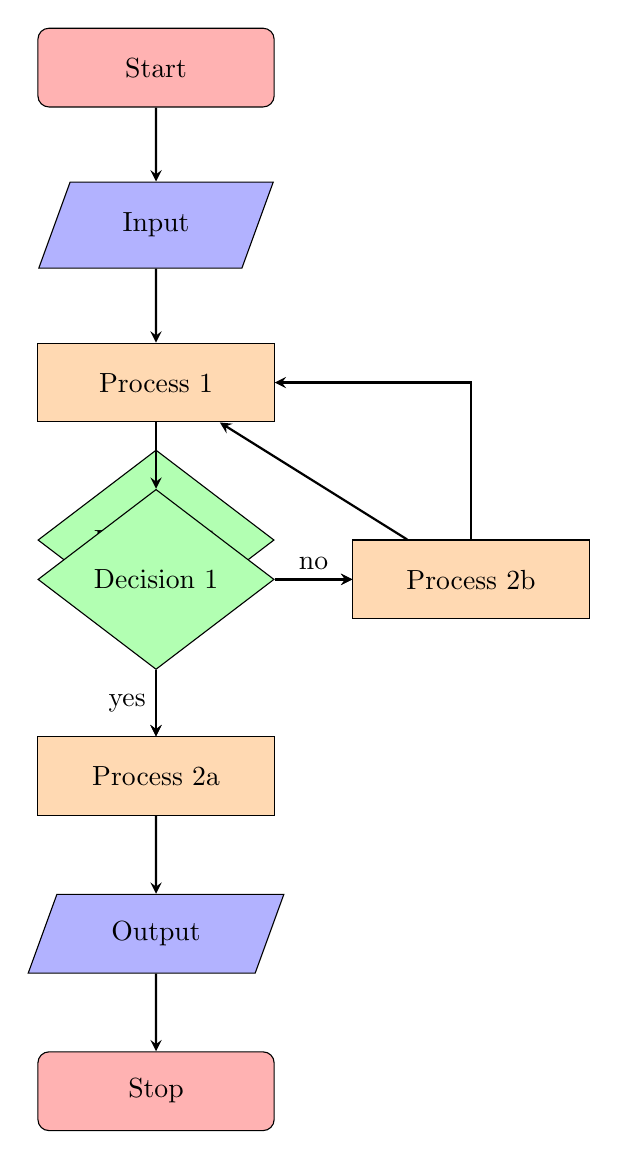
\begin{tikzpicture}[node distance=2cm]
\node (start) [startstop] {Start};
\node (in1) [io, below of=start] {Input};
\node (pro1) [process, below of=in1] {Process 1};
\node (dec1) [decision, below of=pro1] {Decision 1};
\node (dec1) [decision, below of=pro1, yshift=-0.5cm] {Decision 1};
\node (pro2a) [process, below of=dec1, yshift=-0.5cm] {Process 2a};
\node (pro2b) [process, right of=dec1, xshift=2cm] {Process 2b};
\node (out1) [io, below of=pro2a] {Output};
\node (stop) [startstop, below of=out1] {Stop};
\draw [arrow] (start) -- (in1);
\draw [arrow] (in1) -- (pro1);
\draw [arrow] (pro1) -- (dec1);
\draw [arrow] (dec1) -- (pro2a);
\draw [arrow] (dec1) -- (pro2b);
\draw [arrow] (dec1) -- node[anchor=east] {yes} (pro2a);
\draw [arrow] (dec1) -- node[anchor=south] {no} (pro2b);
\draw [arrow] (pro2b) -- (pro1);
\draw [arrow] (pro2a) -- (out1);
\draw [arrow] (out1) -- (stop);
\draw [arrow] (pro2b) |- (pro1);
\end{tikzpicture}
\end{frame}

\begin{frame}
\smartdiagram[priority descriptive diagram]{
  Develop a document structure,
  Choose a document class,
  Select suitable packages,
  Setup the document preamble,
  Write your document,
  Finetune the layout}
\end{frame}

\begin{frame}
\begin{center}
\smartdiagram[bubble diagram]{
Build a program,1,2,3,Modify~/\\ Add,5, 6,7
}
\end{center}
\end{frame}

\begin{frame}
\smartdiagramset{set color list={blue!40!yellow, blue!40!orange, blue!40!red, blue!40!purple, blue!40!gray}}
\tikzset{priority arrow/.append style={rotate=180,anchor=0,xshift=30,}}
\smartdiagram[priority descriptive diagram]{yellow, orange, red, purple, blue}
\end{frame}

\begin{frame}
\begin{columns}[T] % align columns
\begin{column}{.48\textwidth}
\color{red}\rule{\linewidth}{4pt}
\smartdiagramset{set color list={blue!40!yellow, blue!40!orange, blue!40!red, blue!40!purple, blue!40!gray}}
\tikzset{priority arrow/.append style={rotate=180,anchor=0,xshift=30,}}
\smartdiagram[priority descriptive diagram]{yellow, orange, red, purple, blue}
\end{column}%
\hfill%
\begin{column}{.48\textwidth}
\color{blue}\rule{\linewidth}{4pt}

\smartdiagramset{set color list={blue!40!yellow, blue!40!orange, blue!40!red, blue!40!purple, blue!40!gray}}
\tikzset{priority arrow/.append style={rotate=180,anchor=0,xshift=30,}}
\smartdiagram[priority descriptive diagram]{yellow, orange, red, purple, blue}
\end{column}%
\end{columns}
\end{frame}

\begin{frame}{The minipage environment}
\begin{minipage}{0.47\textwidth}
    \begin{itemize}
        \item First item
        \item Second item
        \item Third item
    \end{itemize}
\end{minipage}
\resizebox{5.0cm}{!}{%
    \smartdiagramset{set color list={blue!40!yellow, blue!40!orange, blue!40!red, blue!40!purple, blue!40!gray}}
\tikzset{priority arrow/.append style={rotate=180,anchor=0,xshift=30,}}
\smartdiagram[priority descriptive diagram]{yellow, orange, red, purple, blue}
}%
\end{frame}

% \begin{frame}
%  \centering
%  \begin{figure}
%    \only<1-3>{
%        \begin{subfigure}[b]{0.3\textwidth}
%          \caption{Free Positioning}
%                \includegraphics[width=\textwidth,height=\textwidth]{./png/crio}
%                \label{fig:guided}
%                \setcounter{subfigure}{0}% Reset subfigure counter
%        \end{subfigure}\hfill
%        }
%    \only<2-3>{
%        ~ %add desired spacing between images, e. g. ~, \quad, \qquad etc.
%          %(or a blank line to force the subfigure onto a new line)
%        \begin{subfigure}[b]{0.3\textwidth}
%        \setcounter{subfigure}{1}% Reset subfigure counter
%          \caption{Neural Network}
%                \includegraphics[width=\textwidth,height=\textwidth]{./png/cri}
%                \label{fig:free}
%        \setcounter{subfigure}{0}% Reset subfigure counter
%        \end{subfigure}\hfill
%        }
%    \only<3-3>{
%        ~ %add desired spacing between images, e. g. ~, \quad, \qquad etc.
%          %(or a blank line to force the subfigure onto a new line)
%        \begin{subfigure}[b]{0.3\textwidth}
%            \setcounter{subfigure}{2}% Reset subfigure counter
%          \caption{Matlab Output}
%                \includegraphics[width=\textwidth,height=\textwidth]{./png/pod}
%                \label{fig:multiple}
%        \end{subfigure}%
%        }
%        \caption{Different wireless charging approaches~\label{fig:animals}}
%  \end{figure}
%  \begin{itemize}[<+->]
%      \item<1-| alert@1> Free positioning charging based on Inductive coupling~\cite{wireless}.
%      \item<2-| alert@2> Based on RLoad and Frequency Input and Output~\cite{wireless}. %\ref{fig:free}
%      \item<3-| alert@3> Simulation of Matlab Output based on RLoad as an Input~\cite{wireless}. %   \ref{fig:multiple}
%  \end{itemize} 
%\end{frame}

	% \section{Summary}
\subsection{Key points repetition}

\begin{frame}
\setbeamercovered{dynamic}
	\begin{exampleblock}{Summary}
		\begin{itemize}[<+->]
			\item In section~``\nameref{sec:k8sFuntamentals}'' page ``\ref{sec:k8sFuntamentals}'' Container Run Time Interfaces.
			\item In section~``\nameref{sec:k8sVagrant}'' page ``\ref{sec:k8sVagrant}'' Problems / Desires / Solutions on CI / CD.
			\item In section~``\nameref{sec:implementation}'' page ``\ref{sec:implementation}'' CI / CD Flow Build / Deploy / Test. \pause
		\end{itemize}
	\end{exampleblock}
	\begin{exampleblock}{Extra Notes}
		\begin{itemize}[<+->]
			\item Demo on CI / CD build / deploy / validation and error handling cases.
			\item Both the CI / CD and Kubernetes project are provided as open source contribution. The Presentation was written in \alert{\LaTeX}
		\end{itemize}
	\end{exampleblock}
\end{frame}

\subsection*{Questions}
\begin{frame}
%\begin{overlayarea}{\textwidth}{3cm}
    %\only<1>{Some text for the first slide.\\Possibly several lines long.}
    %\only<2>{Replacement on the second slide.}
%\end{overlayarea}
	\begin{center}
		\Huge \textcolor{cyan}{\emph{Coming up: Q \& A}}
	\end{center}
\end{frame}
	% \include{./bibliography/bibliography}
\end{document}
